%%%%%%%%%%%%%%%%%%%%%%%%%%%%%%%%%%%%%
% This is a template file for trying to make boxes, minipages, etc.

\documentclass[pagesize=auto]{scrbook}

\usepackage{comment}
\usepackage{etoolbox}
\usepackage{fancyvrb}
\usepackage{graphicx}
\usepackage{hyperref}
\usepackage[round]{natbib}
\usepackage{xspace}
\usepackage{xcolor}

% This is for multilingual work. Would be nice to support Chinese and Thai.
\usepackage[T2A]{fontenc}
\usepackage[utf8]{inputenc}
\usepackage[greek,russian,english]{babel}
\usepackage{amsthm}
\usepackage{amsmath}
\usepackage{amssymb}
\usepackage[linesnumbered,algoruled,boxed,lined]{algorithm2e}
\usepackage{hyperref} % This package is needed for \texorpdfstring

% This file is for commands / macros / functions.

% That at least was the original intention. As you can see from the comments, some of the commands
% that work for TeX and pdf output are innefective when applied to HTML and eBooks!

% These are useful because HTML output corrupts the result of the \latex command.
\newcommand{\latex}{LaTeX\xspace}
\newcommand{\tex}{TeX\xspace}

% Makes extra space in HTML but not in PDF output.
\def\htbr{\ifdefined\HCode{\HCode{<br/><br/>}}\fi}

\newcommand\nextpage[1][]{
\ifdefined\HCode {
  \HCode{<mbp:pagebreak />}}
\else
  \newpage
\fi
}

% Makes small typewriter text, comparable to other font sizes.
\def\smalltt#1{\texttt{\small #1}}

% Makes small verbatim inline typewriter text, comparable to other font sizes.
% Use as \sverb|My verbatim text|
\def\sverb{\Verb[fontsize=\small]}

% Makes small URL text, comparable to other font sizes.
\def\surl#1{{\small{\url{#1}}}}
\newtheorem{theorem}{Theorem}
\newtheorem{definition}{Definition}
\newtheorem{lemma}{Lemma}
\newtheorem{proposition}{Proposition} 
\newtheorem{corollary}{Corollary} 
\newtheorem{remark}{Remark}


\begin{document}

Hello outside a box!

\begin{center}
Hello outside a box, centered!
\fbox{Hello in a box, centered!}
\end{center}

\begin{figure}
  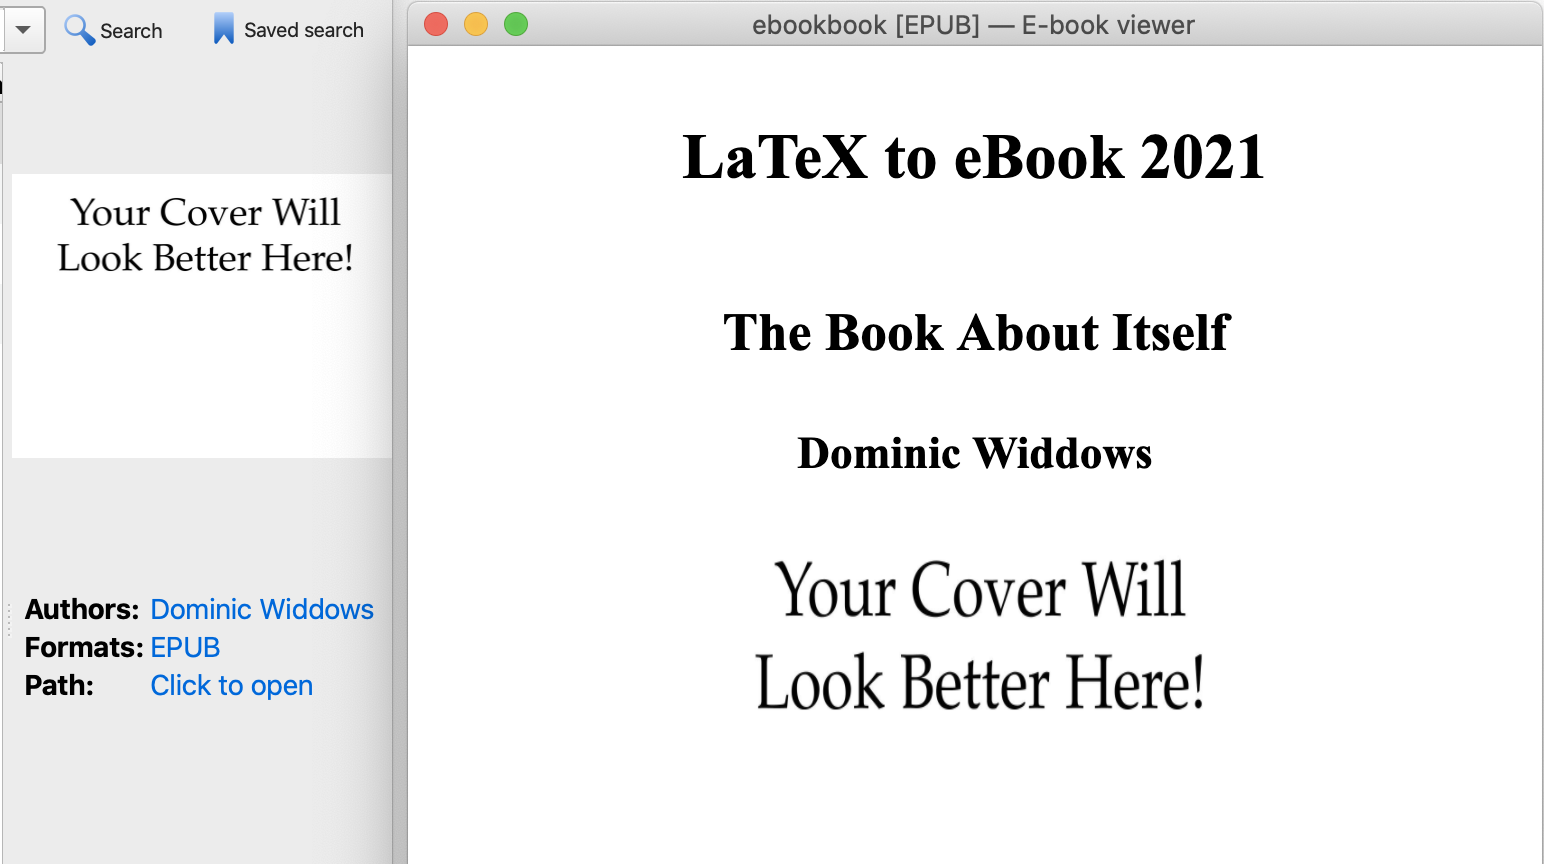
\includegraphics[width=0.5\linewidth]{../../images/calibre_screenshot.png}
  \caption{Screenshot in a figure but not a box}
\end{figure}

\begin{center}
\begin{figure}
  \begin{center}
  \fbox{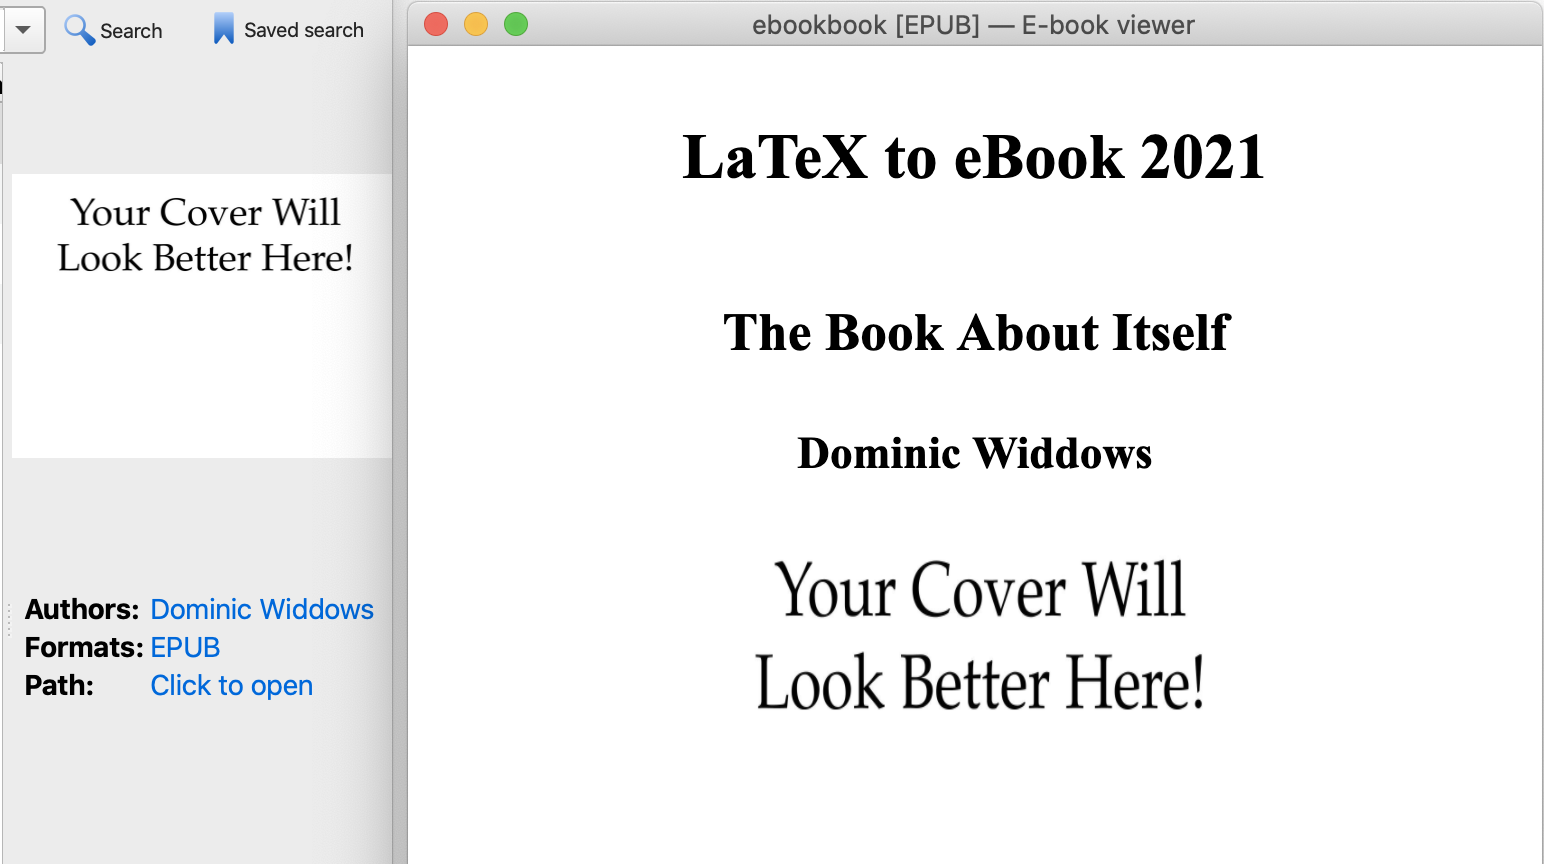
\includegraphics[width=0.5\linewidth]{../../images/calibre_screenshot.png}}
  \caption{Screenshot in an fbox in a figure - floats to the left, however often I try to center it}
  \end{center}
\end{figure}
\end{center}

\begin{figure}
    \begin{minipage}{0.6\textwidth}
        \makebox[0.4\columnwidth][l]{line1}
        \par
        \makebox[0.4\columnwidth][l]{line2}
        \par
        \makebox[0.4\columnwidth][r]{line3}
    \end{minipage}
    \begin{minipage}{0.375\textwidth}
        \centering 
        %\includegraphics{pic.jpg}
        image
    \end{minipage}
\end{figure}

So what's the problem?

\end{document}
